\chapter*{Preamble}
The point of these notes is to introduce the main concepts of calculus using what is known as little-$o()$ notation, in the hope to provide a perspective that is simple, expressive, intuitive and correct.

\section*{Algebra is essential}
\marginnote{Stitz-Zeager [\url{www.stitz-zeager.com}] and Boundless [\url{www.boundless.com}] are good backgrounds references.}
I assume you are comfortable with algebra, including working with rational algebraic expressions, exponents and logarithms, function notation, absolute values, and inequalities.

For example, seeing 

\begin{equation*}
f(x)=\frac{x^2+1}{x^2-1}
\end{equation*}
\begin{marginfigure}
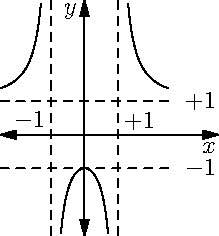
\includegraphics[width=0.75\linewidth]{graphics/algebra1.pdf}
\caption{$y=f(x)=\frac{x^2+1}{x^2-1}$}
\label{fig:algebra1}
\end{marginfigure}

And being asked to show
\begin{equation*}
    f(x+h)=\frac{x^2+1}{x^2-1}+ \frac{2h\cdot(2x+h)}{(x-1)(x+1)(x+h+1)(x+h-1)}
\end{equation*}
\begin{marginfigure}
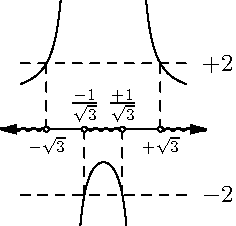
\includegraphics[width=0.75\linewidth]{graphics/algebra2.pdf}
\caption{Where $|f(x)|$ is less than $2$.}
\label{fig:algebra2}
\end{marginfigure}
and
\begin{align*}
  |f(x)|<2 & \text{ if and only if } \\
           &  x \in (-\infty,-\sqrt{3})\cup(-\frac{1}{\sqrt{3}},+\frac{1}{\sqrt{3}})\cup(+\sqrt{3},+\infty)
\end{align*}
should seem (at worst) tedious, but not mysterious.  Neither should the following:
\begin{equation*}
    2^{\log_3(x)}=x^{\log_2(3)} \,.
\end{equation*}
\begin{marginfigure}
\includegraphics[width=0.75\linewidth]{graphics/explog.pdf}
\caption{How $y=2^x$ and $x=\log_2 y$ are related.}
\label{fig:explog}
\end{marginfigure}

If these are mysterious to you, then you need to learn college algebra.
\section*{Trigonometry is helpful}

Additionally, it would be nice if you have some basic trigonometry, including measuring angles in radians, which is the only unit of angle we care about here.  For example,
\begin{gather*}
    (\cos a)^2 +(\sin a)^2 = 1\,,\\
    \cos a=
        \frac{1}{2}\text{ if and only if $a=\pm\frac{\pi}{3}+2n$, for some integer $n$}\,,
\intertext{and}
    \sin(a+b)=\sin(a) \cos(b)+\cos(a) \sin(b)\,,
\end{gather*}
\begin{marginfigure}
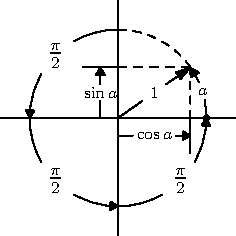
\includegraphics[width=0.75\linewidth]{graphics/unitcircle.pdf}
\caption{Defining $\cos a$ and $\sin a$ for radian angle $a$ on the unit circle.}
\label{fig:unitcircle}
\end{marginfigure}
should at least be familiar to the point of looking something up to remember the details.

\section*{Reading Tips}
\begin{itemize}
\item Focus. The best environment for learning something mathematical is in a small group willing to help you work out a sudoku puzzle.  If you can't work out a sudoku puzzle in the place and with the people you study with, you will not learn mathematics.  You are also not a multi-tasker: you might multitask (usually poorly) on things you already understand; this is something you are trying to understand.
\item Drive, don't walk. Learning to use a computer algebra system can spare you from a lot of tedium compared to a crummy calculator.  Wolfram Alpha, Maxima, Maple, and Mathematica are all good choices.
\item Understand first. Proofs are less important than understanding.  If you are mostly interested in the applications of calculus, don't worry as much about understanding every proof.  Concentrate instead on understand why the facts that are shown make sense and how you mights use these facts.  If you are interested in mathematics itself, understanding the proofs are important, but pretty useless without an understanding of why they make sense and how to use them.
\end{itemize}
